\begin{figure*}[t]
\centering
\begin{tikzpicture}[
		triangle/.style = {regular polygon, regular polygon sides=3 },
    node rotated/.style = {rotate=180},
    border rotated/.style = {shape border rotate=180}
	]
	%\node[label=above:{Document image}] (page) {\includegraphics[width=3cm]{images/page_top.png}};
	\node[rounded corners=3pt, label=above:{Detector scores}] (SIFT)
	{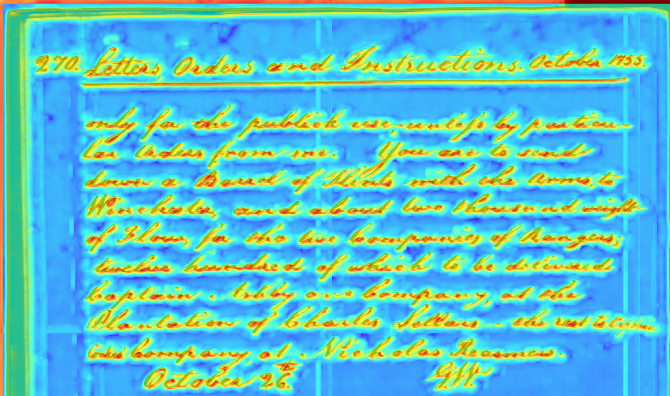
\includegraphics[width=5.1cm]{images/aam-sift_output_overlay0_5_top.png}};
	\node[right=of SIFT, rounded corners=3pt, label=above:{Word hypotheses}] (ER-hyp)
	{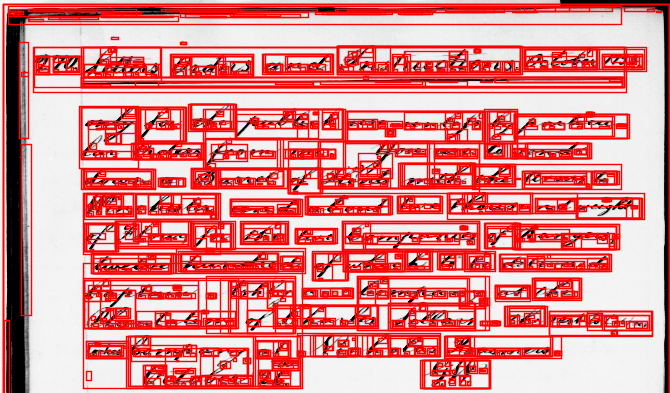
\includegraphics[width=5.1cm]{images/sift_regions_top.png}};
	\node[right=of ER-hyp, rounded corners=3pt, label=above:{Retrieval result}] (ret)
	{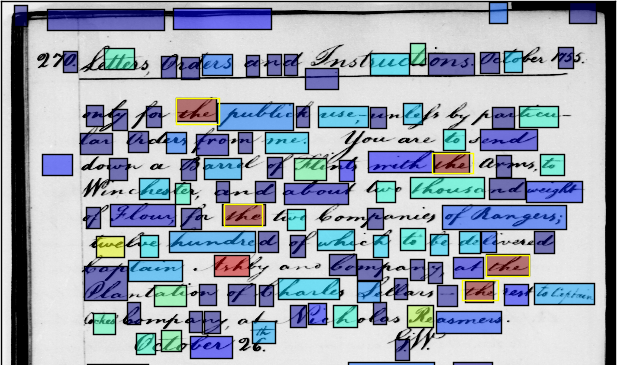
\includegraphics[width=5.1cm]{images/retrieval_the_top.png}};
	\node[node distance=1.5cm, below=of SIFT, rounded corners=5pt, minimum width=5.1cm, label=above:{Query},
	draw](Query){\includegraphics[width=1.8cm]{images/gw/keyb_mac_wide.png}\hspace{1em}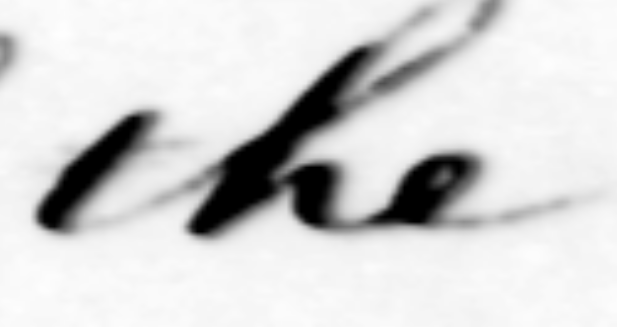
\includegraphics[width=2.4cm]{images/gw/query_2700270_the_168.png}};
	%\node[below=of PHOCNet, draw](filtering){Filtering};
	\node[ellipse, xshift=1.5cm, draw](SIM) at (Query -| ER-hyp) {Similarity};
	\node[text width=2.3cm,align=center, draw](P-NMS)at (SIM -| ret) {Non-maximum suppression};
	\node[above=0.5cm of SIM, triangle, border rotated,inner sep=3pt, draw](AR){};
	\draw[->, >=stealth] (Query) -- (SIM) node[midway, anchor=north, outer sep=4pt, inner sep=2pt, fill=green!20] {PHOC}; 
	\draw (ER-hyp.south -| AR) -- (AR) node[midway, anchor=west, outer sep=4pt, inner sep=2pt, fill=green!20] {PHOC};
	\draw[->, >=stealth] (AR) -- (SIM); 
	\draw[->, >=stealth] (SIM) -- (P-NMS) -- (ret); 
	\draw[dashed] (Query.north east) -- (Query.north east |- AR) -- (AR) node [midway,
	anchor=south]{Aspect ratio filter};
	\draw[->, >=stealth] (SIFT) -- (ER-hyp);
   \end{tikzpicture}
	 \caption{Word hypotheses for segmentation-free word spotting. Text detector scores indicate
	 document image regions in a soft manner.
%	 , modeling the uncertainty of the detection. 
	 Scores are shown with a heatmap visualization in blue to red colors. Based on
	 the scores word hypotheses are extracted using extremal regions. Each hypothesis is
	 represented with a PHOC and its bounding box. At query time, suitable hypotheses are
	 obtained after aspect ratio filtering. The aspect ratio filter is depicted with a triangle. 
	 Afterwards, the similarity between the query PHOC and
	 word hypothesis PHOCs is computed. The retrieval result is obtained after non-maximum
	 suppression of the word hypotheses with respect to similarity with the query. The ranking 
	 %of the retrieved word hypotheses 
	 is visualized with blue (dissimilar) to red (similar) colors.
 }
 \label{fig:overview}
\end{figure*}
